%!TEX root = ../dokumentation.tex

\chapter{Theoretische Grundlagen}\label{cha:Grundlagen}
Für das bessere Verständniss des Themas soll dieses Kapitel die relevanten, theoretischen Grundlagen vermitteln,  und an das Kernthema herranführen. Dabei wird zunächst geklärt, worum es sich bei der Überwachung von IT-Infrastrukturen handelt, und soll Antworten auf Fragen wie "`Warum werden diese überwacht?"', "`Welche Komponenten sind zu unterscheiden?"' und "`Welche Technologien werden eingesetzt?"' geben. Danach soll der Begriff Logfiles genauer definiert werden, bevor die Funktionalität von MapReduce und Hadoop erläutert wird.

%TODO: Einleitung überarbeiten
<Einleitung in das Kapitel noch nicht wirklich rund. Überarbeiten!>

%Kurze Einleitung in das Kapitel. Beschreiben warum die Grundlagen notwendig sind. Auch darüber schreiben, dass nicht ALLE Grundlagen sondern lediglich die für das Verständnis der Arbeit notwendigen erklärt werden.

\section{Überwachung von IT-Infrastrukturen}\label{sec:UeberwachungIT}
Ziel der Überwachung ist es, durch extraktion von Informationen und überprüfen von Komponenten, Aussagen über den Zustand einer oder mehrerer Komponenten innerhalb einer IT-Infrastruktur zu erhalten. Die durch die Überwachung erhobenen Basis-Informationen werden zur Optimierung der Performance und Verfügbarkeit eines Dienstes eingesetzt.

Nach Salm gibt es drei Arten von Komponenten die es zu unterscheiden gilt:

\begin{itemize}
	\item Netzwerk, um eine ausreichende Bandbreite und bestehende Übertragung zu sichern
	\item Ressourcen, um eine effiziente Lastverteilung innerhalb der Infrastruktur zu gewährleisten
	\item Anwendung, um Anwender schnellen, unkomplizierten Zugriff zu ermöglichen
\end{itemize}

Überwachungssysteme zeigen Administratoren die Up- und Downtime, sowie die Auslastung, von Soft- und Hardware an.\footcite[Vgl.][S. 8]{Salm.2007}

Um Aussagen über den Zustand einer Komponente treffen zu können, analysiert das Überwachungssystem eine Vielzahl von Informationen. Dabei werden unterschiedliche techniken eingesetzt von einfachen Standard-Unix-Kommandozeilen-Tools bis hin zu inteligenten Agenten.

Diese Agenten werden auf der Zielkomponente installiert und sind als Hintergrundanwendung dauerhaft aktiv um immer die aktuellsten Informationen an das Überwachungssystem zu übermitteln.

Um eine hohe Qualität der Daten zu gewährleisten, werden die Agenten, entweder direkt oder über eine externe Schnittstelle, so konfiguriert, dass sie nur die Informationen ermitteln und übertragen, welche für das Überwachungssystem relevant sind. Agenten können auch eine direktere Rolle bei der Überwachung von Komponenten übernehmen, indem sie, anstatt oder zusätzlich zu den Informationen, die Daten selbst interpretieren, um Meldungen an das Überwachungssystem zu übermitteln.

In beiden fällen kombinieren Agenten selbst ermittelte Informationen mit bereits vorhandenen. Zu den selbst ermittelten Daten gehören unter anderem CPU und RAM Auslastung oder offene Ports. Bereits vorhandene Informationen können durch auf der Komponente laufende Software, oder durch die Komponente selbst, erzeugt werden.

%TODO: Überleitung zu Logfiles schreiben aus fokusieren auf web und monitoring systemen
<Kurze Fokusierung auf Online Service. Welche Informationen werden hier im speziellen benötigt. Erwähnen von Monitoring Systemen. Funktion von Agenten, im zusammenspiel mit Monitoring Systemen, bei der analyse von Logfiles beschreiben und daraus die Überleitung zu Logfiles ableiten>

%Worum geht es bei der Überwachung? Was ist das Ziel? Warum braucht man eine Überwachung? Wie sieht diese i.d.R. Aus? Welche Kernpunkte gibt es in der Überwachung? \\
%Hier sollte die Überleitung zum nächsten Kapitel kommen d.h. Logfiles werden als letztes behandelt in diesem Kapitel, damit der Übergang sauber ist.

\section{Bedeutung von Logfiles}\label{sec:BedeutungVonLogfiles}
Nach Baur und Blasius bezeichnen Logfiles (oder auch Protokolldateien) \flqq [...] automatisch erstellte Dateien [..], in denen bestimmte Ereignisse elektronisch aufgezeichnet werden.\frqq\footcite[S. 847]{Baur.2014} Dabei werden sowhl negative wie auch positive Ereignisse protokolliert.

Bei Web-Servern, welche mit Apache unter Linux betrieben werden, stellen syslog von Linux, soweie Error- und Access-Log von Apache, die Grundlage zur Überwachung des Servers. Sie lassen sich sehr einfach durch die in \autoref{sec:UeberwachungIT} beschriebenen Agenten überwachen, da sie einem klar vorgegebenen Standard folgen.

Im syslog von Linux werden alle Ereignisse protokolliert, welche im direkten Zusammenhang mit dem System stehen. Die Einträge folgen dabei der im \ac{RFC} 5424\footcite[RFC 5424,][]{RFC5424.2009} festgehaltenen Beschreibung (Da es sich bei RFC um keine offizielle Norm handelt, handelt es sich lediglich um eine Beschreibung, nicht um einen Standard).

Das Apache-Error-Log enthält diagnostische Informationen und protokolliert alle Fehler, welche bei der Verarbeitung einer Anfrage auftreten. \autoref{lst:BeispieleintragApacheErrorLog} zeigt, wie ein Eintrag in einem Error-Log aussehen könnte. Es lässt sich klar erkennen, wann der Fehler aufgetreten ist, was fehlgeschlagen ist und welches Modul betroffen ist. Ebenfalls sichtbar ist die \ac{IP}-Adresse des Clients, bei dem der Fehler aufgetreten ist. Die Einträge des Error-Logs entsprechen keiner Norm oder \ac{RFC} Beschreibung. Sie können nach der Installation individuell angepasst werden.\footcite[Vgl.][]{ApacheErrorLog.2015} \\

\begin{lstlisting}[caption=Beispieleintrag für ein Appache-Error-Log,label=lst:BeispieleintragApacheErrorLog]
[Fri Jun 12 10:42:29.902022 2015] [core:error] [pid 35708:tid 4328636416] [client 192.168.172.15] File does not exist: /usr/local/apache2/htdocs/favicon.ico
\end{lstlisting}

Im Apache-Access-Log werden alle Anfragen an den Server protokolliert. Dabei wird gespeichert von welcher \ac{IP}-Adresse die Anfrage kam, wann die Anfrage gestartet wurde, welcher art die Anfrage war und welche Pfad angefragt wurde, sowie welcher Statuscode zurückgegeben wurde und wie groß die Antwort des Server war (siehe \autoref{lst:BeispieleintragApacheAccessLog}). \\

\begin{lstlisting}[caption=Beispieleintrag für ein Appache-Access-Log,label=lst:BeispieleintragApacheAccessLog]
192.168.172.15 - Max [11/Jun/2015:13:55:36 -0700] "GET /dummy.gif HTTP/1.0" 200 2326
\end{lstlisting}

Wie beim Error-Log können die Einträge angepasst werden und folgen somit keiner Norm oder \ac{RFC}. Die Beispiele zeigen ebenfalls, wie unterschiedlich die Einträge für zwei Logfiles des gleichen Systems sein können.\footcite[Vgl.][]{ApacheAccessLog.2015}

%TODO: Gesetz zur Vorratsdatenspeicherung suchen und abgleichen mit TMG und BDSG
Da es sich bei \ac{IP}-Adressen potenziell um Personenbezogenen daten handelt, ist diese nach §3 Abs. 1 des \ac{BDSG} geschützt\footcite[§3 Abs. 1 BDSG,][]{BDSG3.1990} (Potenziell Personenbezogen, da nicht ersichtlich ist ob eine \ac{IP}-Adresse sttisch oder dynamisch ist). Die speicherung der \ac{IP}-Adresse ist daher nur gestattet, wenn der Anwender zustimmt, oder ein Grund für die speicherung vorliegt, welcher §15 \ac{TMG} genügt.\footcite[§15 TMG,][]{TMG15.2007} Ist dies nicht der Fall, darf die \ac{IP} nicht Teil des Protokolleintrags sein. Die Standardeinstellung muss entsprechend verändert werden.

Aufgrund der Gesetzeslage, muss die im Zuge dieser Arbeit entwickelte Anwendung, bei der Weiterverarbeitung der Daten, den gesetzlichen Vorlagen genügen. Dabei ist besonders zu beachten, ob eine Anonymisierung oder Pseudonymisierung der Daten stattfinden muss. Dieser Aspekt wird in \autoref{cha:Planung} näher betrachtet.

%TODO: Kapitel Logfiles zusammenfassen und aus nicht norm folgenden notation überleitung zu MapReduce bilden
<Zusammenfassung am ende des Kapitels. Aufzeigen das Logfiles unterschiedliche Notation besitzen und keinem einheitlichen Standard folgen. Erwähnen das die üblichen Logs trotz allem durch Agenten auswertbar sind, die Logs um die es später geht jedoch nicht. Aus dieser Aussage die verwendung von MapReduce begründen und daraus die Überleitung zu MapReduce bilden>

%Was sind Logfiles im allgemeinen? Was ist die Funktion eines Logfiles? Gibt es Standards? Wenn ja welche und wie sehen die aus? Werden die Standards im weiteren Verlauf der Arbeit noch einmal relevant sein (Ja/Nein begründen und erläutern)?

%TODO: Kapitel inhaltlich abgeschlossen. Review für Formuliereungen und Rechtschreibung noch offen. Auch auf überleitungen zu den unterkapiteln achten um lesefluss nicht zu stören
\section{Einführung in MapReduce}\label{sec:EinführungInMapReduce}
Die Google Mitarbeiter Jeffrey Dean und Sanjar Ghemawat veröffentlichten 2004 eine Arbeit, in welcher sie einen neuen Ansatz zur Verarbeitung von großen, unstrukturierten Daten beschrieben. Das in der Arbeit beschriebene Modell wurde als \textit{Map-Reduce} bezeichnet. Dabei wurde nicht nur beschrieben, wie man große Datenmengen durchsucht, auswetet und in Schlüssel-Wert-Paaren zusammenfast. Die Clusterung von Jobs auf \gls{Commodity-Hardware} waren ebenfalls ein Bestandteil der Arbeit. Freiknecht schreibt weiter, dass diese Arbeit als Ursprung des Algorithmus bezeichnet wird, und somit Implementierungen wie Hadoop, Disco oder BashReduce inspiriert hat.\footcite[Vgl.][S. 42]{Freiknecht.2014}

Ein MapReduce Programm lässt sich i.d.R. in drei Bereiche unterteilen. Der Map-Phase, in welcher die Schlüssel-Wert-Paare aus den Eingabedaten erzeugt werden, der Combine-Phase, zur Aggregation der Paare, sowie der Reduce-Phase, in welcher die Daten ausgedünnt werden, bis nur noch ein Wert pro Schlüssel vorhanden ist (siehe \autoref{fig:DreiPhasenMapReduce}).

\begin{figure}[h]
	\centering
	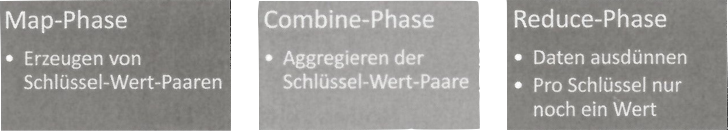
\includegraphics[width=.8\textwidth]{MapReduce_001.png}
	\caption{Die drei Phasen eines Map-Reduce-Prozesses\footnotemark}
	\label{fig:DreiPhasenMapReduce}
\end{figure}
\footnotetext{\cite[S. 42.]{Freiknecht.2014}}

Die Stärke von MapReduce, liegt in der Kombination von sequentieller und paralleler Verarbeitung. Die einzelnen Phasen von MapReduce werden sequentiell ausgeführt. Die Combine- oder Reduce-Phase kann nicht beginnen, bevor die Map-Phase abgeschlossen ist. Innerhalb der Phasen können die Aufgaben jedoch auf mehrere Instanzen verteil und parallel verarbeitet werden. Diese Form der Verarbeitung entspricht dem Master-Worker-Modell.\footcite[Vgl.][S.1 f]{Karloff.2010}

Speziell bei der Parallelisierung von Tasks, welche wenig bis keine Abhängigkeit voneinander aufweise, stellt dieses Modell ein ideales Hilfmittel dar. Die zentralen Elemente des Shemas bildet ein Master und $n$ Worker. Der Master startet die Verarbeitung, indem er ein gegebenes Probelm aufarbeitet und eine Sammlung von Tasks erzeugt.  Die Tasks werden vom Master an die ihm bekannten Worker verteilt (Worker werden entweder vom Master selbst erzeugt oder melden sich bei diesem an). Die Worker arbeiten parallel und senden einen Statuscode an den Master, sobald der Task vollständig bearbeitet wurde (oder der Worker in einen Fehler läuft).\footcite[Vgl.][S. 80 ff]{Fey.2008} \autoref{fig:MasterWorkerInMR} zeigt die Anwendung des Master-Worker-Modells auf ein MapReduce Programm.

\begin{figure}
	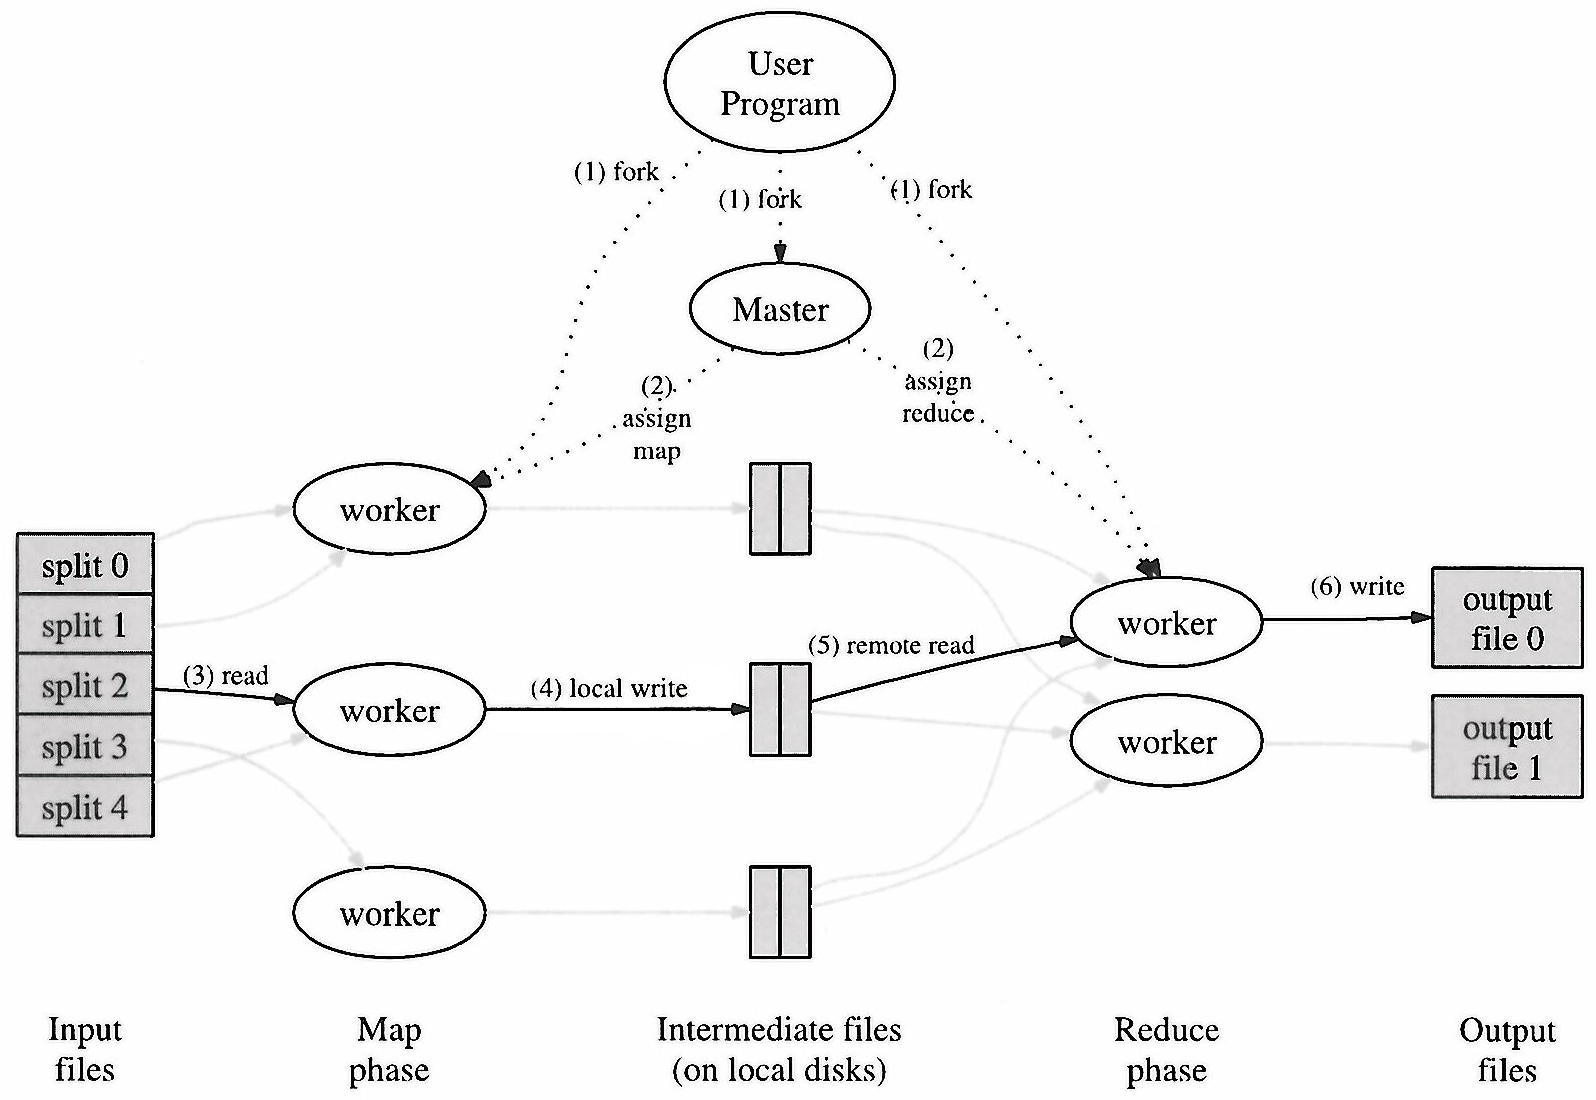
\includegraphics[width=1\textwidth]{MasterWorkerMR.png}
	\caption{Master-Worker in MapReduce\footnotemark}
	\label{fig:MasterWorkerInMR}
\end{figure}
\footnotetext{\cite[S. 3.]{Dean.2004}}

Im folgenden wird MapReduce zunächst formal definiert. Die Grundlage der Definition bildet das durch Karloff, Suri und Vassilvitskii beschriebene \ac{MRC} Model.\footcite[S. 3 f]{Karloff.2010} Danach soll die Funktionsweise anhand eines Beispiels weiter verdeutlicht werden.

\subsection{Formale Beschreibung von MapReduce}\label{subsec:FormaleBeschreibung}
Da es sich bei MapReduce um ein Modell zur Verarbeitung von Daten handelt, und nicht um einen Algorithmus, wird die durch Karloff et al. beschriebene \ac{MRC} verwendet, um eine Grundlage für die formale Definition zu haben. Dabei werden die drei Karakteristiken Funktion, Ausführungszeit und Speicherauslastung beschrieben.

Im zentrum der Datenverarbeitung mit MapReduce steht das Schlüssel-Wert-Paar, welches als ein String Tupel $\langle k; v \rangle$, mit dem Schlüssel $k$ und dem dazu gehörenden Wert $v$. Die Eingabe für eine \ac{MRC} Maschiene ist eine Liste von Schlüssel-Wert-Paaren $\langle k_i, v_i \rangle_{i=1}^{\mathbb{N}}$ mit einer Gesamtgröße im Speicher von $\sum_{i=1}^{\mathbb{N}}|k_i|+|v_i|$.

Die Map Funktion verarbeitet einen Tupel $\langle k; v \rangle$ zu einer Liste von neuen Schlüssel-Wert-Paaren $\langle k_1; v_1 \rangle, \langle k_2; v_2 \rangle, \dots, \langle k_n; v_n \rangle$.

Die Reduce Funktion erhält als Eingabeparameter einen Schlüssel $k$ sowie eine Sequenz von Werten $v_1, v_2, \dots, v_n$. Aus diesen erzeugt die Funktion eine Liste von Schlüssel-Wert-Paaren $\langle k; v_{k,1} \rangle, \langle k; v_{k,2} \rangle, \dots, \langle k; v_{k,n} \rangle$. Die Schlüssel der Tupel in der erzeugten Liste ist identisch mit dem Schlüssel, welcher an die Reduce Funktion übergeben wurde.

Aus diesen beiden Definitionen folgt, dass die Map Funktion Schlüssel nach belieben manipulieren kann. Für Reduce sind die Schlüssel jedoch unveränderlich.

Die Ausführung von MapReduce lässt sich wie folgt deifnieren. Sei $M$ die Menge aller Map und Reduce Funktionen $\langle \mu_1, \rho_1, \mu_2, \rho_2, \dots, \mu_R, \rho_R \rangle$ und $U_0$ eine Liste von Tupeln $\langle k; v \rangle$, dann gilt für die Ausfürhung von $M$ auf die Daten $U_0$:

Für $r = 1, 2, \dots, R$:

\begin{enumerate}
	\item \textbf{MAP:} $\forall \langle k; v \rangle \in U_{r-1}$ führe $\mu_r \in M$ mit $\langle k; v \rangle$ aus. Die Funktion erzeugt eine Liste neuer Tupel $\langle k_1; v_1 \rangle, \langle k_2; v_2 \rangle, \dots, \langle k_n; v_n \rangle$. Sei $U_r^{\prime}$ die Ausgabe für eine Eingabe $\langle k; v \rangle$, dann gilt: $U_r^{\prime} = \bigcup_{\langle k; v \rangle \in U_{r-1}} \mu_r(\langle k; v\rangle)$.
	\item \textbf{COMBINE:} $\forall k$ erzeuge Liste $V_{k,r}$ mit den Werten $v_i$, so dass gilt $\langle k; v_i \rangle \in U_r^{\prime}$.
	\item \textbf{REDUCE:} $\forall k$, übergebe $k$ und eine willkürliche Permutation von $V_{k,r}$ in eine Instanz von Reducer $\rho_r \in M$ zur Ausführung. Dieser erzuegt eine Liste von Tupeln $\langle k; v_1^{\prime} \rangle, \langle k; v_2^{\prime} \rangle, \dots, \langle k; v_n^{\prime} \rangle$. Sei $U_r$ die Ausgabe für die Eingabe $\langle k; V_{k,r} \rangle$, \\ dann gilt: $U_r = \bigcup_k \rho(\langle k; V_{k,r}\rangle)$.
\end{enumerate}

Die Verarbeitung wird beendet, wenn der letzte Reducer $\rho_R$ beendet wird. In der Definition wird die Möglichkeit zur Parallelisierung, der sequentiell ausgeführten Funktionen Map und Reduce deutlich. Sowohl Mapper als auch Reducer verarbeiten immer nur einen Tupel zeitgleich. Es können also mehrere Instanzen von $\mu_r$ und $\rho_r$ gestartet werden.\footcite[Vgl.][S. 2 f]{Karloff.2010}

Die Ausfürhungszeit von MapReduce kann nicht spezifiziert werden ohne ein wissen über den Inhalt der Funktionen. Die Effizient hängt von den in den Funktionen angewandten Algorithmen ab. Allgemein lässt sich folgende Ausführungszeit definieren: Teilt man die Map-Phase in $M$ teile und die Reduce-Phase in $R$ teile, dann lässt sich allgemein eine Ausführungszeit von $O(M+R)$ festlegen. Für die Speicherauslastung gilt dabei eine maximale Auslastung von $O(M \ast R)$.\footcite[Vgl.][S. 5]{Dean.2004}

\subsection{Beispielanwendung von MapReduce}\label{subsec:Beispielanwendung}
Die formale Definition von MapReduce soll nun anhand eines einfachen Beispiels verdeutlicht werden. Dazu wird auf eine Beispielanalyse aus dem Buch "`Hadoop - Zuverlässig, verteilte und skalierbare Big-Data-Anwendungen"' von Ramon Wartala zurückgegriffen.

In seinem Beispiel will Wartala aufzeigen, wie, ohne die volle Funktionalität der Hadoop-Api zu nutzen und unter Verwendung von Standard-Unix-Kommandozeilen-Tools wie \textit{grep}, \textit{sort}, \textit{cat} und \textit{awk}, aus einer CSV-Datei eine spezifische Information extrahiert werden kann.

\autoref{tbl:Beispieldaten} zeigt die in seinem Beispiel verwendeten Daten. Dabei handelt es sich um die Anzahl der im Hafen Hamburg von 2004 bis 2011 umgeschlagenen Container pro Monat. Um die Verarbeitung für das Beispiel zu vereinfachen, wurde aus den Daten eine dreispaltige CSV-Datei erzeugt im Vormat \textit{Jahr;Monat;Container-Umschlag}.

\begin{table}[h]
	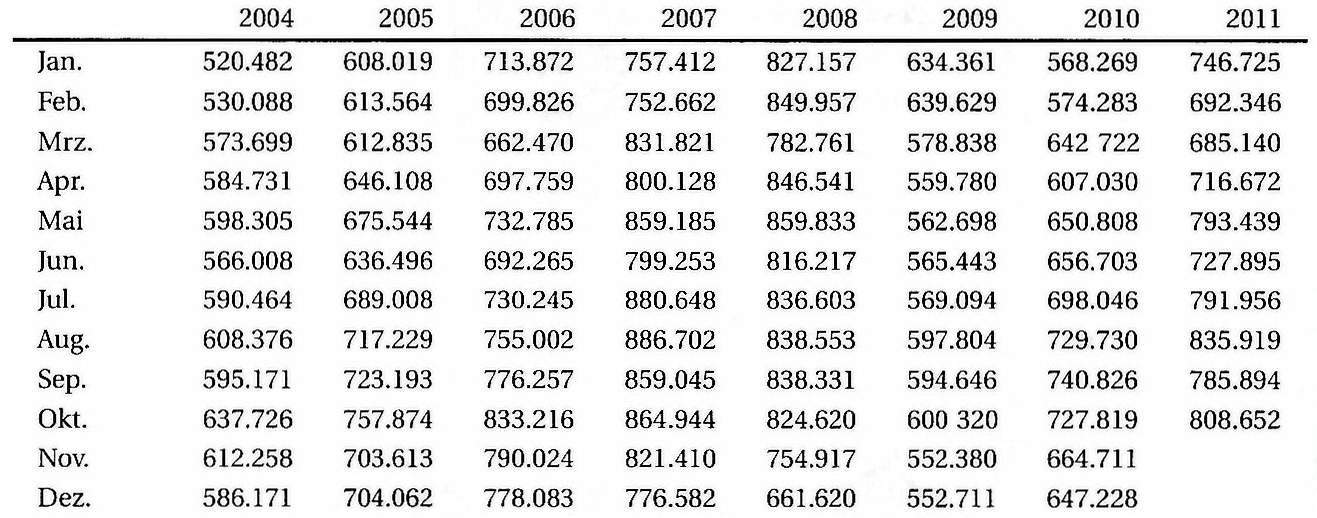
\includegraphics[width=1\textwidth]{Beispieldaten.png}
	\caption{Beispieldaten: Anzahl umgeschlagener Container\footnotemark}
	\label{tbl:Beispieldaten}
\end{table}
\footnotetext{\cite[S. 26.]{Wartala.2012}}

Die Information, welche mit MapReduce ermittelt werden soll, ist der Monat im Jahr 2004 mit den meisten umgeschlagenen Containern. Dieser Task lässt sich, unter Verwendung der erwähnten Unix-Tools, in drei Teilaufgaben seperieren. Als erstes werden mit den \textit{grep}-Befehl alle Zeilen ausgegeben, welche aus dem Jahr 2004 stammen (siehe \autoref{lis:Grep2004}). Dieser Schritt repräsentiert den Mapper für dieses Beispiel. \\

\begin{lstlisting}[language=bash, caption={Befehl zur Anzeige aller Zeilen mit Jahr 2004\protect\footnotemark}, label=lis:Grep2004]
grep 2004
\end{lstlisting}
\footnotetext{\cite[S. 27.]{Wartala.2012}}

Danach werden die Zeilen nach der dritten Spalte sortiert (Spalten wurden mit ; getrennt, siehe \autoref{lis:SortiereZeilen}). Dieser Befehl repräsentiert die Combine-Phase des Modells. \\

\begin{lstlisting}[language=bash, caption={Befehl zur Sortierung der Zeilen nach der dritten Spalte\protect\footnotemark}, label=lis:SortiereZeilen]
sort -t ';' -k +3 -r
\end{lstlisting}
\footnotetext{\cite[S. 27.]{Wartala.2012}}

Zuletzt wird die maximale Anzahl der Container bestimmt und das Jahr sowie der Monat und die Anzahl ausgegeben (siehe \autoref{lis:AusgabeBeispiel}). Dieser letzte Schritt in diesem Beispiel steht für den Reducer. \\

\begin{lstlisting}[language=bash, caption={Ausgabe des Beispielprogramms\protect\footnotemark}, label=lis:AusgabeBeispiel]
awk 'max== "" || $3 > max {max=$3;jahr=$1;monat=$2} END { print "jahr:" jahr; print "monat:" monat; print "anzahl:" max;}' FS=";"
\end{lstlisting}
\footnotetext{\cite[S. 27.]{Wartala.2012}}

Mit Hilfe der Unix-Befehls-Pipeline lassen sich alle Befehle auf eine Zieldatei Anwenden (siehe \autoref{lis:VollständigerBefehl}). Das Ergebnis wird in die Datei maximum\_umschlag.txt geschrieben.\footcite[Vgl.][S. 26 ff]{Wartala.2012} \\

\begin{lstlisting}[language=bash, caption={Vollständiger Befehl zur Auswertung der Beispieldaten\protect\footnotemark}, label=lis:VollständigerBefehl]
cat container_umschlag.csv | grep 2004 | sort -t ';' -k +3 -r | awk 'max== "" || $3 > max {max=$3;jahr=$1;monat=$2} END { print "jahr:" jahr; print "monat:" monat; print "anzahl:" max;}' FS=";" | cat > maximum_umschlag.txt
\end{lstlisting}
\footnotetext{\cite[S. 28.]{Wartala.2012}}

Hier wird deutlich, dass es sich bei MapReduce nicht um einen Algoritmus, sondern um ein Vorgehensmodell handelt. Es geht lediglich darum, die Datenverarbeitung so effizient wie möglich sowohl parallel als auch seriell durchzuführen. Wie das Beispiel zeigt, lässt sich dieses Vorgehen auch sehr minimalistisch anwenden.

%TODO: Überleitung zum nächsten Kapitel noch offen
<Noch ein paar sätze zur anwendung auf komplexere daten. Daraus die Überleitung zum nächsten Kapitel über Hadoop und das Framework schaffen>

%Woher kommt MapReduce? Wie funktioniert MapReduce? Stärken/Schwächen aufzeigen. Versuchen den Algorithmus mathematisch zu beschreiben ($O(n)$ Methode, Mengenleere). Hierfür muss noch Literatur gesucht werden. Bisher nur mathematische Beschreibungen im Internet gefunden.

\section{Was ist Hadoop?}\label{sec:WasIstHadoop}
\flqq Kurz gesagt: Hadoop ist ein freies, Java-basiertes Open-Source-Framework für die skalierbare und verteilte Verarbeitung großer Datenmengen auf vielen Rechnern innerhalb eines Netzwerks.\frqq\footcite[S. 21]{Wartala.2012}

Die Entwicklung begann im Jahr 2004 durch den Programmierer Doug Cutting, nachdem dieser, im Rahmen des 6. Symposiums \textit{Operating Systems Design and Implementations} (\acs{OSDI}), den Vortrag "`MapReduce - Simplified Data Processing on Large Clusters"', von den Google Mitarbeitern Jeffrey Dean und Sanjay Ghemawat, gehört hatte.

Zu diesem Zeitpunkt arbeitete Cutting an seinem Suchmaschienenprojekt mit dem Namen "`Nutch"', welches bereits 2002 ins leben gerufen wurde. Sein Ziel war eine leistungsfähige und konkurrenzfähige Softwarearchitektur, die es mit kommerziellen Suchmaschienen aufnehmen konnte. Bis 2004 konnte Nutch bereits 100 Mio. Webseiten mit nur vier Rechnerknoten indexieren.

Um jedoch das gesamte World Wide Web indexieren zu können, suchte Cutting gemeinsam mit der Nutch-Community nach einer Möglichkeit, die zugrundeliegende Architektur noch skalierbarer zu machen. Nach dem Vortrag bei der \acs{OSDI} fand Cutting eine passende Systemarchitektur in einem ebenfalls durch Dean und Ghemawat veröffentlichten Ansatz.\footcite[Näheres siehe][]{Dean.2004}

Gemeinsam mit zwei Teilzeit-Programmierern implementierte er ein, durch das Google Dateisystem \ac{GFS} inspiriertes, verteiltes Dateisystem, um darauf den MapReduce-Ansatz unter Nutch zu realisieren. 2006 wechselte Cutting zu Yahoo!. Das Dateisystem und MapReduce-Framework wurde aus Nutch extrahiert und in das eigenständige Apache-Projekt Hadoop überführt. Heute wird Hadoop in einer Reihe von Unternehmen produktiv eingesetzt, darunter Yahoo!, IBM und Microsoft.\footnote{Referenzzahlen für Unternehmen, die Hadoop einsetzen, unter:\\ \url{http://wiki.apache.org/hadoop/PoweredBy}}

Hadoop besteht aus zwei Kernkomponenten. Dem verteilten Dateisystem \ac{HDFS} und dem MapReduce-Framework. Dabei wird keine spezielle Servertechnik benötigt. Hadoop lässt sich sehr leicht auf Standardhardware betreiben.\footcite[Vgl.][S. 19-22]{Wartala.2012}

Die einzlenen Komponenten sind unabhängig voneinander einsetzbar. Eine große Rolle spielt bei Hadoop das Konzept der Datenlokalität. Entgegen dem normalen vorgehen, bei welchem einem Programm die daten zu verfügung gestellt werden, wird bei Hadoop das Programm zur Ausführung im Cluster verteilt. Da es sich bei Hadoop i.d.R. um Anwendungen im Big Data bereich handelt, macht es Sinn, da die Anwendung wesentlich kleiner und somit schneller zu übertragen ist, als die Daten.\footcite[Vgl.][S. 20]{Freiknecht.2014}

\subsection{Das verteilte Dateisystem HDFS}\label{subsec:DasVerteilteDateisystemHDFS}
<Was ist ein verteiltes Dateisystem überhaupt und wozu braucht man es? Vergleich mit einem normalen Dateisystem?>

%\subsection{MapReduce-Framework}\label{subsec:MapReduceFramework}
%ACHTUNG. Vermutlich überflüssig da MapReduce bereits beschrieben wurde. Das Framework funktioniert nicht wirklich anders es stellt nur interfaces bereit damit die klassen stimmen.

\subsection{Abgrenzung - Was ist Hadoop nicht?}
<Was gehört alles zu Hadoop? Worauf zieht Hadoop ab? Warum verwende ich Hadoop statt es einfach selbst zu machen? Stärken und Schwächen aufzeigen.>

%\section{Betrachten von Alternativen}
%Alternativen sowohl zu Hadoop als auch zu MapReduce selbst. Was gibt es in diesen Bereichen noch? Wie unterscheiden sich diese?
%TODO: Alternativen in 3.3 und 5.1 oder eher 5.4 betrachten/erwähnen